
\begin{center}
\textbf{\large 2. МОДЕЛЬ ПЛАВЛЕНИЯ ПЕРЕГРЕТЫХ КРИСТАЛЛОВ}
\end{center}
\refstepcounter{chapter}
\addcontentsline{toc}{chapter}{2. МОДЕЛЬ ПЛАВЛЕНИЯ ПЕРЕГРЕТЫХ КРИСТАЛЛОВ}


\section{Введение}

Плавление -- один из наиболее изученных фазовых переходов, важных для атомных, молекулярных, коллоидных и белковых систем.
Однако в настоящее время не существует микроскопических экспериментально доступных критериев, которые можно было бы использовать для надежного отслеживания эволюции системы при переходе, критериев, дающих возможность понять физику зародышеобразования при плавлении и эволюции фронта плавления.
Чтобы решить эту проблему, была разработана теоретическая модель в рамках теории среднего поля с использованием нового локального параметра порядка (экспериментально измеримого) -- нормированного среднеквадратичного смещения между частицами в соседних ячейках Вороного.
Предложенная модель протестирована при помощи компьютерного моделирования при различных режимах динамики частиц (броуновским и ньютоновским).
В результате обнаружено, что данная модель обеспечивает превосходное описание эволюции системы при пересечении линии плавления.

Явление плавления широко распространено в природе и может быть обнаружено, начиная от атомных и молекулярных до белковых и коллоидных систем и выходя далеко за рамки материаловедения, поэтому формулировке критериев плавления в микроскопическом масштабе уделяется значительное внимание уже около 100 лет.
Один из наиболее широко используемых микроскопических подходов принадлежит Линдеману~\cite{lindemann1910}, в частности отметим, его переосмысление Гилварри~\cite{10.1103/physrev.102.308}: то, что сейчас известно как критерий Линдемана -- это утверждение, что плавление происходит, когда среднеквадратичное смещение атомов от их положения достигает определенной доли (обычно 0.1-0.15) межатомного расстояния.
Популярность критерия обусловлена его простотой и интуитивно понятным способом применения, но есть и существенные недостатки, включая низкую точность в прогнозировании температуры плавления и отсутствие явного учета жидкого состояния~\cite{10.1098/rspa.1991.0068}.
Впоследствии, был введен ряд критериев, которые можно проследить до работы Гилварри~\cite{10.1063/1.1426419}, в особенности, с развитием современных экспериментальных и вычислительных методов, которые обеспечивают доступ к смещениям атомов.
Но детали структурных изменений, главным образом в отношении этих критериев, остаются неуловимыми, а ряд ключевых явлений, куда входят детали механизма зародышеобразования, кинетики фронта плавления и поведения системы вблизи точки плавления, остаются малоизученными.


\section{Материалы и методы}

\subsection{$\lambda^2$-Параметр: Локальная мера беспорядка}
\label{SSMF-AppA}

В работе~\cite{10.1021/acs.jpcc.7b09317}, для характеризации локальной разупорядоченности и идентификации конденсированных (жидких или твердых) фаз в конденсируемых системах был предложен подход, основанный на анализе ячеек Вороного -- элементарной площади (''объема''), занимаемой каждой частицей в системе.
В рамках данного подхода на первом этапе система разбивается на ячейки Вороного, чтобы вычислить следующий параметр:
\begin{equation}
\label{SSMF-eq1}
\sigma_{i} =\frac{1}{a_i N_{ni}}\sqrt{\sum_{j<k}^{N_{ni}}{(r_{ij}-r_{ik})^2}/2}, \quad r_{ij}=|\mathbf{r}_i-\mathbf{r}_j|,
\end{equation}
где $\mathbf{r}_i$ -- радиус-вектор $i$-ой частицы, $N_{ni}$ -- количество соседних ячеек, $a_i = \sqrt{S_i/\pi}$ -- характерный радиус, $S_i$ -- площадь ячейки Вороного.
На втором этапе для подавления сильных локальных тепловых флуктуаций проводится усреднение с соседними ячейками, которые имеют общую грань (сторона в 2D случае) с ячейкой частицы $i$ \cite{10.1021/acs.jpcc.7b09317}:
\begin{equation}
\label{SSMF-eq2}
\lambda_{i} = \frac{1}{N_{ni}+1}\left(\sigma_{i}+\sum_{j=1}^{N_{ni}}{\sigma_{j}}\right).
\end{equation}
В результате получается стандартное отклонение $\lambda_i^2$ расстояний между соседними частицами в \emph{физически малом объеме} в окрестности $i$-й частицы.
Важно отметить, что $\lambda_i^2$ одинаково хорошо применимо для характеризации как твердой, так и жидкой фаз системы, поскольку этот параметр связан с локальным беспорядком в физически малом объеме~\cite{10.1021/acs.jpcc.7b09317}.
В кристаллах $\lambda^2$ связано с параметром Линдемана для соседних частиц~\cite{10.1016/0375-9601(85)90617-6}, так как $\lambda^2 \propto \sigma_\|^2$, где $\sigma_\|^2$ -- продольная компонента среднеквадратичного смещения ближайших частиц.


\subsection{Детали моделирования МД}
\label{SSMF-AppC}

Проведено МД-моделирование кристаллов в условиях ланжевеновской динамики.
В качестве характерного примера рассмотрена система частиц, взаимодействующих по обратному степенному закону (IPL18):
\begin{equation}
\label{SSMF-eq3}
\varphi(r) = \epsilon a \left(\frac{\sigma}{r}\right)^{18},
\end{equation}
где $\epsilon$ и $\sigma$ -- сила и характерный масштаб отталкивания соответственно,
а параметр $ a = 2.365 $ введен для удобства моделирования скачкообразного изменения диаметра частиц.
Использовалась нормированная температура $ T/ \epsilon \rightarrow T $, расстояние $ r/ \sigma \rightarrow r $, плотность частиц $\rho\sigma^3/m\rightarrow n$ и время $t\sqrt{\epsilon/m\sigma^2} \rightarrow t$ ($m$ -- масса частицы).

Для анализа плавления перегретого кристалла выполнено МД-моделирование системы, состоящей из $ N = 7.2 \times 10 ^ 4 $ частиц в $NVT$ ансамбле при $n=0.867$ и $T=1$.
В исходном состоянии частицы располагались в ГЦК решетке, ориентированной таким образом, чтобы плоскость (111) совпадала с горизонталью.
Размеры области моделирования в $ x $, $ y $ и $ z $ - направлениях выбраны с учетом $ L_x / L_z \approx 20.4 $ и $ L_y / L_z \approx 21.3 $.
Временной шаг взят равным $ \Delta t = 7.4 \times 10 ^ {- 4} \sqrt {m \sigma ^ 2 / \epsilon}$.
Расчеты методом молекулярной динамики проводились в открытом программном пакете LAMMPS.
Моделирование проводилось в 2 этапа: (i) система моделировалась на протяжении $ 10 ^ 5 $ временных шагов с $ a = 7.224 $ для достижения состояния равновесия; (ii) значение $a$ фиксировалось равным $ 2.365 $ и проводилось дополнительное моделирование на $ 4 \times 10 ^ 5 $ шагов для анализа плавления в кристалле.

\section{Результаты}
\subsection{Самосогласованная модель среднего поля эволюции $\lambda^2$ - поля}

Примеры кристаллических и жидких структур показаны на Рис.~\ref{SSMF-Figure1}(a) и \ref{SSMF-Figure1}(b) соответственно.
Белые точки -- частицы; ячейки Вороного показаны сплошными серыми линиями, и окрашены в соответствии со значением параметра $\lambda^2$ -- нормированным среднеквадратичным смещением между частицами в соседних ячейках Вороного~\cite{10.1021/acs.jpcc.7b09317}.
В кристаллах $\lambda^2$ связано с параметром Линдемана для соседних частиц~\cite{10.1016/0375-9601(85)90617-6}.
Это обусловлено тем, что $\lambda^2\propto \sigma_ \| ^ 2 $, где $ \sigma_ \| ^ 2 $ -- продольная составляющая среднеквадратичного смещения ближайших частиц.
Кроме того, $ \sigma_ \| ^ 2 $ играет важную роль в вычислении первого корреляционного пика в кристаллах \cite{10.1063/1.4869863, 10.1063/1.4926945, 10.1088/0953-8984/28/23/235401, 10.1039/c7sm02429k, 10.1063/1.5116176}.
После плавления кристаллическая решетка разрушается, но, несмотря на диффузию частиц, разбиение Вороного все еще применимо в жидкости.

В случае систем с отталкиванием, рост $\lambda^2$ обеспечивается (i) повышением температуры или (ii) уменьшением плотности.
В то время как первый механизм имеет ключевую роль в системах с мягким отталкиванием между частицами (например, в мягких кристаллах при низких температурах $\lambda^2\propto T $), последний является определяющим в системах типа твердых сфер (таких как коллоиды NIPAm), коллективная динамика которых определяется объемной долей частиц.
В обоих случаях $\lambda^2$ счиатется параметром порядка, и в этих терминах плавление представляет собой переход от состояний с малым $\lambda^2$ (кристалл) к состояниям с большим $\lambda^2$ (жидкость).

Чтобы получить самосогласованную модель эволюции $ \lambda^2$-поля,
необходимо рассмотреть слабо неоднородное пространственное поле $\lambda^2$.
Параметр $\lambda ^ 2$ неконсервативен, следовательно его эволюция определяется нестационарным уравнением Гинзбурга-Ландау (или моделью Ланжевена)~\cite{book.desai}:
\begin{equation}
\label{SSMF-eq4}
\frac{\partial \lambda^2}{\partial t} = -\Gamma \frac{\delta \mathcal{F}}{\delta \lambda^2} + \varepsilon^{1/2}\xi(t,\mathbf{r}),
\end{equation}
где $\Gamma$ -- обобщенная вязкость, $ \mathcal{F} $ -- функционал свободной энергии системы, $\langle \xi(t,\mathbf{r})\xi(t',\mathbf{r}')\rangle = \delta(t-t')\delta(\mathbf{r}-\mathbf{r}')$ и $\varepsilon = 2k_BT\Gamma$.
Последнее слагаемое в~\eqref{SSMF-eq2} описывает тепловые флуктуации поля $\lambda^2$.

\begin{figure}[!t]
\centering
  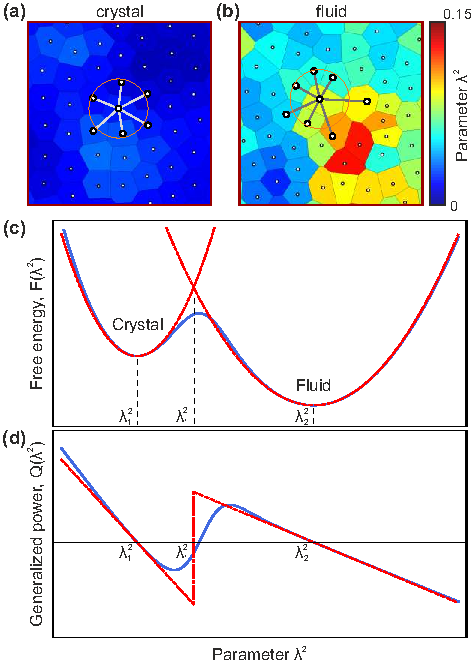
\includegraphics[width=100mm]{SSMF-Figure1.pdf}
  \caption{\textbf{Схематичное изображение к предлагаемой самосогласованной $\lambda^2$~-~модели:}
  (a) и (b) снимки системы в кристаллическом и жидком состоянии (взяты из МД моделирования).
  Ячейки Вороного раскрашены в соответствии со значениями параметра $ \lambda^2$.
  Панели (c) и (d) схематично иллюстрируют (синие линии) зависимость свободной энергии $ F (\lambda ^ 2) $ (в однородной системе) и обобщенную мощность $ Q (\lambda ^ 2) $, сопряженную с полем $\lambda^2$.
  Пунктирные красные линии иллюстрируют ступенчатое приближение \eqref{SSMF-eq5} и \eqref{SSMF-eq7}.
  }
\label{SSMF-Figure1}
\end{figure}


\begin{figure*}[!t]
\centering
  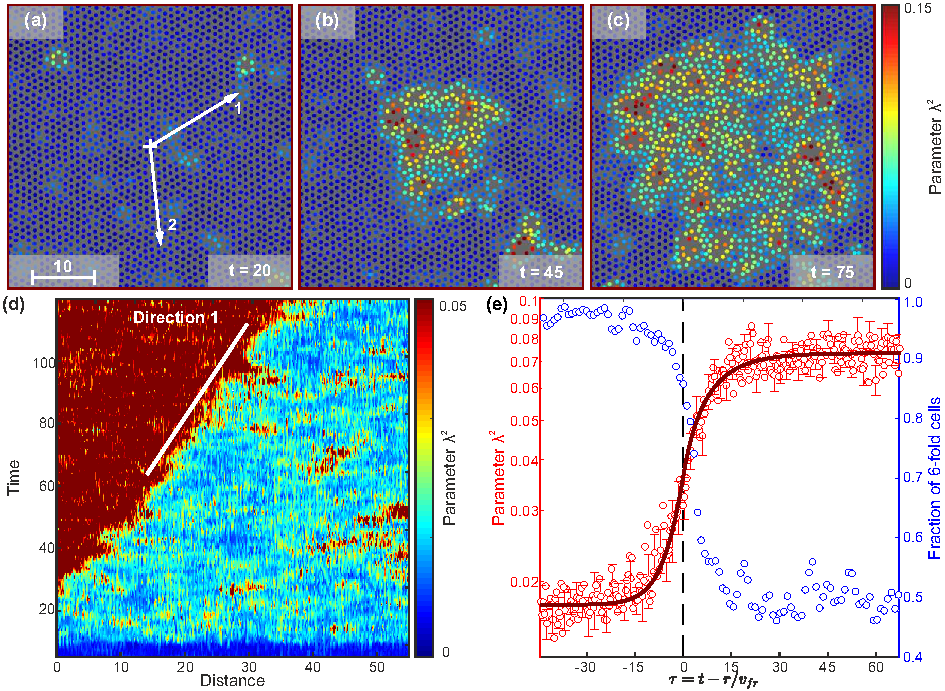
\includegraphics[width=\linewidth]{SSMF-Figure3.pdf}
  \caption{\textbf{Автомодельный $ \lambda^2$-профиль распространяющегося фронта плавления в перегретом кристалле, наблюдаемый при МД-моделировании:}
  (a) - (c) Последовательные снимки системы, где круги представляют собой частицы, окрашенные в соответствии со значением $\lambda^2$.
  (d) Эволюция поля $\lambda^2(r, t)$ в радиальном направлении (1), показанном на (a).
  (e) $\lambda^2(\tau)$ -- профиль распространяющегося фронта плавления при росте зародышей.
  Красные символы -- экспериментальные точки, красная сплошная линия -- теоретическая аппроксимация \eqref{SSMF-eq9}.
  Синие символы представляют собой долю ячеек Вороного с 6-ю соседями в плоскости анализа, а резкое падением, указывает на разрушение кристаллической структуры.}
\label{SSMF-Figure3}
\end{figure*}

Функционал свободной энергии $\mathcal{F}[\lambda^2] = \int{d\mathbf{r}\;F[\lambda^2]}$ в квадратичном приближении может быть представлен в виде:
\begin{equation}
\label{SSMF-eq5}
F[\lambda^2] = F_{\mathrm{1,2}}^{(0)}+\frac{1}{2}A_{1,2}\left(\lambda^2-\lambda_{1,2}^2\right)^2 + \frac{1}{2}\alpha_{1,2}\left(\nabla\lambda^2\right)^2,
\end{equation}
где $F_{1,2}^{(0)}$ -- энергия однородного состояния ($1$ или $2$), $A$ и $\alpha$ -- положительные коэффициенты разложения \cite{book.desai}, а индексы $ 1 $ и $ 2 $ соответствуют кристаллическому или жидкому состоянию при $\lambda^2 \lessgtr \lambda_\ast^2$ соответственно.
Параметр $\lambda_\ast^2 $ -- это порог, связанный с обобщенным критерием плавления типа Линдемана, предполагается, что $ F_{\mathrm{1}} ^ {(0)}> F_{\mathrm{2}} ^ {(0)}$ для рассматриваемого случая.

При помощи уравнений~\eqref{SSMF-eq4} и \eqref{SSMF-eq5} можно получить:
\begin{equation}
\label{SSMF-eq6}
\frac{\partial \lambda^2}{\partial t} = \chi_{1,2} \nabla^2\lambda^2 + Q(\lambda^2) +  \varepsilon^{1/2}\xi(t,\mathbf{r}),
\end{equation}
где $ \chi_{1,2} = \alpha_{1,2} \Gamma$ характеризует диффузию $\lambda^2$,
а $ Q (\lambda ^ 2) $ -- обобщенный источник $ \lambda^2$-поля,
\begin{equation}
\label{SSMF-eq7}
Q(\lambda^2) =
\left\{
  \begin{array}{ll}
  -\gamma_{1}\left(\lambda^2-\lambda_{1}^2\right), & \lambda^2  < \lambda_\ast^2;\\
  -\gamma_{2}\left(\lambda^2-\lambda_{2}^2\right), & \lambda^2 > \lambda_\ast^2,\\
  \end{array}
\right.
\end{equation}
где $\gamma_{1,2} = \Gamma A_{1,2}$.
Уравнение \eqref{SSMF-eq6} демонстрирует аналогию с эволюцией температуры в химически реактивных средах \cite{10.1088/0004-637x/805/1/59} и совпадает с уравнением для кинетической температуры, которое исследовалось в работах~\cite{10.1103/physreve.96.043201, 10.1103/physreve.97.043206, 10.1103/physreve.100.023203} при анализе распространяющихся фронтов неравновесного плавления в однослойных пылевых плазменных кристаллах.

Энергия \eqref{SSMF-eq5} для однородного случая и соответствующая обобщенная мощность $ Q (\lambda ^ 2) $ показаны на Рис.~\ref{SSMF-Figure1}(с) и \ref{SSMF-Figure1}(d).
Как видно на Рис.~\ref{SSMF-Figure1}(d), система может существовать долгое время в окрестности устойчивых состояний с $\lambda^2= \lambda_{1,2} ^ 2 $, тогда как пороговое значение $\lambda^2=\lambda_\ast^2$ соответствует неустойчивой точке.
Ниже показано, что решение уравнения~\eqref{SSMF-eq6} объясняет два важных явления, изучаемых в настоящем исследовании:
(i) распространение автомодельных фронтов плавления в перегретых кристаллах, образованных частицами, движущимися в броуновском или ньютоновском динамическом режиме, и (ii) бифуркационное поведение различных $\lambda^2$ -флуктуаций (зародышей плавления) в перегретом кристалле.

Если пренебречь влиянием теплового шума и полагать кривизну фронта плавления незначительной при его распространении, то это означает, что $ \epsilon \simeq 0 $ и в уравнении~\eqref{SSMF-eq6} можно записать $ \nabla ^ 2 = \partial ^ 2 / \partial r ^ 2 $.
В этом случае, самоподобный профиль (бегущей волны плавления) описывается функцией $\lambda^2(t-r/v_\mathrm{fr})\equiv \lambda^2(\tau)$ (где $v_\mathrm{fr}$ -- скорость фронта), которая подчиняется уравнению:
\begin{equation}
\label{SSMF-eq8}
\frac{\chi_{1,2}}{v_{\mathrm{fr}}^2} \frac{d^2 \lambda^2}{d\tau^2} -\frac{d \lambda^2}{d \tau} -\gamma_{1,2}(\lambda^2-\lambda_{1,2}^2) =0,
\end{equation}
учитывая, что $\lambda^2(\tau) $ и его производная $ d\lambda^2/ d \tau $ должны быть непрерывными в точке $ \tau = 0 $, где $\lambda^2=\lambda_\ast^2$.
Полученное уравнение идентично уравнению, которое возникает в задаче неравновесного плавления в комплексных (пылевых) плазменных кристаллах, следовательно, решение уравнения~\eqref{SSMF-eq8} аналогично \cite{10.1103/physreve.96.043201, 10.1103/physreve.100.023203}:
\begin{equation}
\label{SSMF-eq9}
\frac{\lambda^2(\tau)-\lambda^2_1}{\lambda^2_\ast-\lambda^2_1}=
\left\{
  \begin{array}{ll}
    e^{p_1 \tau}, & \tau < 0;\\
    1+\left(1-e^{-p_2\tau}\right)p_1/p_2 , & \tau > 0,\\
  \end{array}
\right. \\
\end{equation}
где $ p_{1,2} = \left(\sqrt {1 + 4 \gamma_{1,2} \chi_{1,2} / v_\mathrm{fr} ^ 2} \pm 1 \right) v_\mathrm{fr} ^ 2/2 \chi_{1,2} $ -- показатели в экспоненциальных ветвях решения до и после фронта плавления.
В пределе $\tau \gg 1$, $\lambda^2(\tau) \rightarrow \lambda_2^2$, откуда следует, что
$\left(\lambda_2^2-\lambda^2_1\right)/\left(\lambda^2_\ast-\lambda^2_1\right) = (1+p_1/p_2)$.
Скорость фронта плавления и показатели $p_{1,2} $ (неизвестные \emph{априори}) сложным образом определяются диффузией $\lambda^2$, спецификой межчастичных взаимодействий и различием химических потенциалов на границе жидкость-твердое тело~\cite{10.1038/ncomms7942}.


\subsection{Прямое наблюдение автомодельного профиля стационарных фронтов плавления в МД симуляции}
\label{SSMF-Results-MD}

Распространение фронтов плавления -- медленный процесс по сравнению с характерным временем движения отдельных частиц.
Это означает, что описание в терминах медленно флуктуирующего $\lambda^2$-поля должно быть применимым как в коллоидах, демонстрирующих броуновский режим движения отдельных частиц, так и в системах с ланжевеновской динамикой.
Чтобы подтвердить, что все ключевые особенности, наблюдаемые в случае коллоидных систем, присутствуют и в атомарных кристаллах, было выполнено моделирование аналогичного процесса методом МД с термостатом Ланжевена и слабым затуханием.
При параметрах выполненного МД-моделирования плотность системы при плавлении и кристаллизации (в безразмерных единицах) составляет $ n_m = 0,93 $ и $ n_f = 0,88 $, соответственно~\cite{10.1080/00268979500100911}.
Следовательно, ступенчатое изменение диаметра частиц в проведенных расчетах можно оценить как $ (n_f / n) ^ {1/3} -1 \simeq 0.5 \% $ ($ n = 0.867 $), что позволяет вычислить падение эффективной объемной доли частиц относительно ее значения, соответствующего плавлению:
$\Delta \phi  \simeq (n_m/n)^{1/3}-1\simeq 2.4\%$.
Полученное значение близко к режиму промежуточного перегрева, обсуждаемому в работе~\cite{10.1038/ncomms7942}.


Результаты проведенного МД-моделирования автомодельных фронтов \\ плавления в перегретом кристалле частиц с IPL18 взаимодействием представлены на Рис.~\ref{SSMF-Figure3}.
Полученные значения $\lambda^2$ в кристаллическом, жидком и пороговом состояниях равны $\lambda_1^2 \simeq 0.01$, $\lambda_2^2 \simeq 0.07$, и $\lambda_\ast^2 \simeq 0.035$, соответственно.
Значения $\lambda_\ast^2$, полученные в МД моделированиях хорошо согласуются с критерием Линдемана для ближайших соседей \cite{10.1016/0375-9601(85)90617-6}.


\section{Заключение главы}

Поведение поля $\lambda^2$ было проанализировано с использованием нестационарного уравнения Гинзбурга-Ландау с тепловым шумом и источниками.
Показано, что разработанная модель демонстрирует существенно нелинейное поведение, в то время как слагаемые в уравнениях имеют ясный физический смысл в контексте анализа плавления кристаллов.
Кроме того, будучи по своей сути микроскопической, предложенная модель позволяет с высокой степенью детализации изучать зародышеобразование в различных режимах перегрева (в зависимости от величины теплового шума) и эволюцию реалистичных жидких зародышей, которые могут принимать самые разные сложные формы.

Процесс зародышеобразования в перегретых кристаллах, кинетика образования и роста жидких зародышей и структура устойчивых фронтов плавления являются центральными проблемами для понимания плавления кристаллов.
Представленные результаты являются существенным шагом вперед, предоставляя простой и эффективный инструмент для изучения процессов зародышеобразования и плавления в перегретых кристаллах различной природы.
